% pdflatex new.tex %
\documentclass{article}

\usepackage{graphicx}

\title{C++ Parallel application for Traveling Salesman Problem resolution by genetic algorithm}
\author{Berti Stefano}
\date{\today}

\begin{document}
    \thispagestyle{plain}
    % Titles %
    \begin{center}
        \Large
        \textbf{C++ Parallel application for Traveling Salesman Problem resolution by genetic algorithm}

        \vspace{0.4cm}
        \large Parallel and distributed system: paradigms and models
        \\2019 / 2020

        \vspace{0.4cm}
        \textbf{Berti Stefano}

        \vspace{0.9cm}
        \textbf{Abstract}
    \end{center}
    % Abstract %
    The aim of this project is to implement a genetic algorithm for the resolution of the Traveling Salesman Problem and to parallelize it with two different mechanism:
    \begin{itemize}
	\item C++ standard threads and mutex
	\item Fastflow library
    \end{itemize}


    \section{Problem description}\label{sec:s1}
        The genetic algorithm mimin the natural evolution and selection. In order to do that, we need a population, a way to understand which elements of the population
	will surivive (and so will reproduce), how they reproduce and how mutations can occour.
	\begin{itemize}
	    \item \textbf{Population}: is a matrix (vector of vector), where each row contains a sequence of number, and each number represent a node
	    \item \textbf{Affinity}: for each element x is the probability that x will be selected for reproduction, and is calculated as the inverse of the path length,
	        normalize w.r.t. all other elements in order to obtain a proper probability
	    \item \textbf{Reproduction}: 2 paths A and B can create a new path C by generating 2 random numbers i and j and putting the subsequence B[i, j] in A
	    \item \textbf{Mutation}: a mutation occour with a certain probability to every generated path, and it is a random shuffle of two position in the paths.
		The probability that a mutation does not occour is 0.9.
	\end{itemize}
	To calculate the length of each path, I use a random generated city, where for each node number we have the relative coordinates. The city can also be plotted for
	real time problem resolution visualization, but this has heavy consequences on the program performances.


    \section{A first approach}\label{sec:s2}
	The first approach that i though was a pipeline with feedback composed by a farm for calculting the length of each path, a collector to compute sum and to normalize
	each path length in order to obtain probability, and another farm for the reproduction stage
    \begin{figure}
        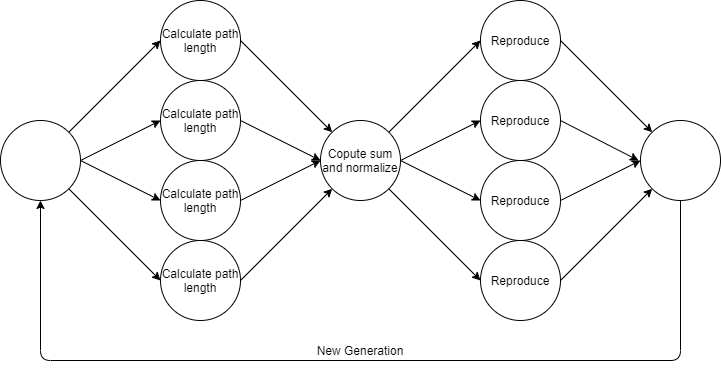
\includegraphics[width=\linewidth]{img/first.png}
        \caption{The first approach}
        \label{fig:first}
    \end{figure}
    but this apporach lead to a poor speedup, because we need to calculate all length paths and to sum them in order to normalize and get probability to use in the reproduce task. But we can think to a different solution, which drive us to the normal form: when the population is big, the probabilities are all small and not very different, if we assume to have more than one independent populations, we will not make the same computation as before because we are not considering anymore the possibility of crossover among all the elements of the population, but our throughtput will increase and our overall population will have the same size as before.

    \section{The second approach}\label{sec:s3}
	This approach is a simple farm of composition of the sequential stage "evolve", which is a combination of the two stages "calculate affinities" and "reproduce"
    \begin{figure}
        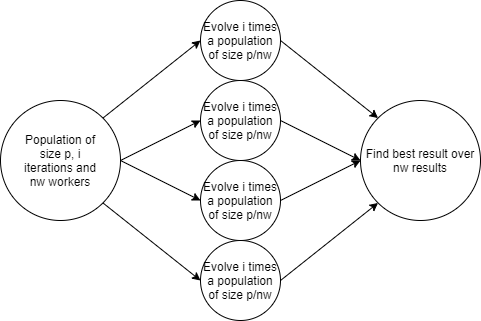
\includegraphics[width=\linewidth]{img/second.png}
        \caption{The second and final approach}
        \label{fig:second}
    \end{figure}
    this computation model is also known as normal form, and it is teorically the best way to set out computation. The resulting speedup is more than linear because as the population gets smaller, the pick\_candidate function has less element to get (for example, with a population of 10000, it spends around 30ms, while with a population of 20000 it spends around 50/60ms). So by parallelizing, we are not only reducing the number of times that we need to create a new member of the population in the main loop, but we are also reducing the time needed to cerate one of them! This will lead to a superscalar speedup, which is not motivated by our hardware, but by the way we implemented the function which select an elements given all elements prpbabilities.


    \section{Performance: local analisy}\label{sec:s4}
	Because of the fact that with the farm we don't reduce only the number of elements of the population that we need to generate at each iteration, but also the time spent to generate each one of them, the times and speedup that we obtain are more than linear, how can be ween in the picture
    \begin{figure}
        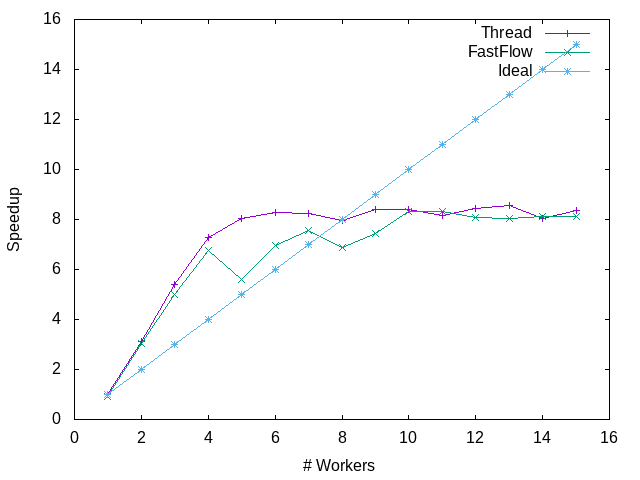
\includegraphics[width=\linewidth]{img/local_20_10000_100_p.png}
        \caption{Local speedup with 20 nodes, 10000 elements of population and 100 iterations}
        \label{fig:local_speedup}
    \end{figure}
    \begin{figure}
        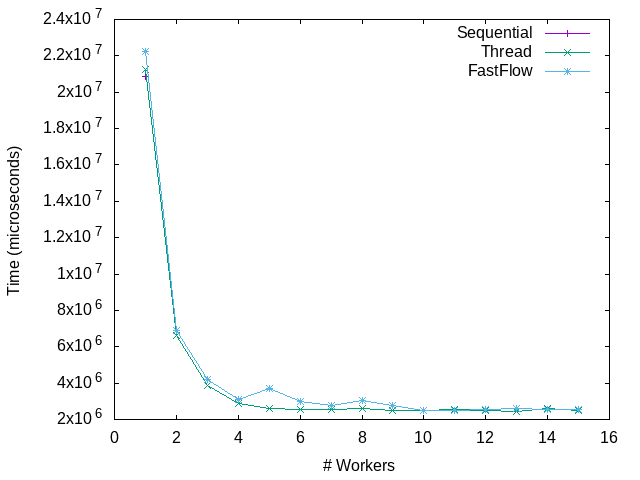
\includegraphics[width=\linewidth]{img/local_20_10000_100_p_t.png}
        \caption{Local time with 20 nodes, 10000 elements of population and 100 iterations}
        \label{fig:local_time}
    \end{figure}
	This case is not easy to analyze, so I modify the code in order to spend O(1) time for the creation of a new element (instead of O(n) in the worst case) by just selecting a random element instead to look to probabilities vector. In this way, the farm has a service time that is what we expected: in the sequential version we have that the population data structure, which is a vector of vector of int, has size 0.8MB (4 byte(int) * 20 * 10000) and the affinities vector has size 0.08MB (8 byte(double) * 10000), and my caches L1, L2, L3 have sizes 9MB, 1.5MB and 0.35MB respectively, so we alwaysfit the L2 caches and with 3 workers, we have a superlinear speedup due to the fact that the data structures fit the L3 cache (the city data structure has negligible dimension, around 20*8*2 byte). I have 5 core in my virtual machine, so the knee is set around 5 workers. The service time of the farm is max{Tw/nw, Tsched, Tgat}, but the scheduler only has to read the parameters from command line, and the gatherer has to see all the nw results to select the best path among them, but the number of workers is low (<<100), so the heaviest part of the computation is let to the worker. We have that our sequential time is 7568352 usec, with threads and 1 worker is 7626354 usec and with fastflow and one worker is 8088780 usec, so they all are very similiar. The thread implementation, like the fastflow implementation implements a simple farm, so the service time is reduced like the expectation, and the thread implementation is a little better because it does not use external library and it is simpler
    \begin{figure}
        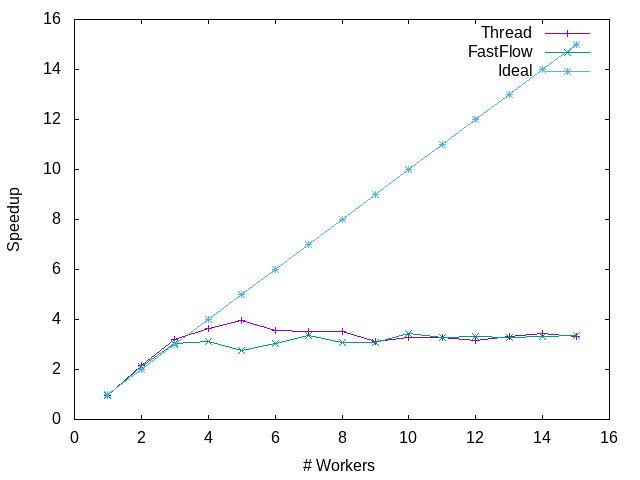
\includegraphics[width=\linewidth]{img/local_20_10000_100_rand.png}
        \caption{Local speedup with 20 nodes, 10000 elements of population and 100 iterations}
        \label{fig:local_speedup}
    \end{figure}
    \begin{figure}
        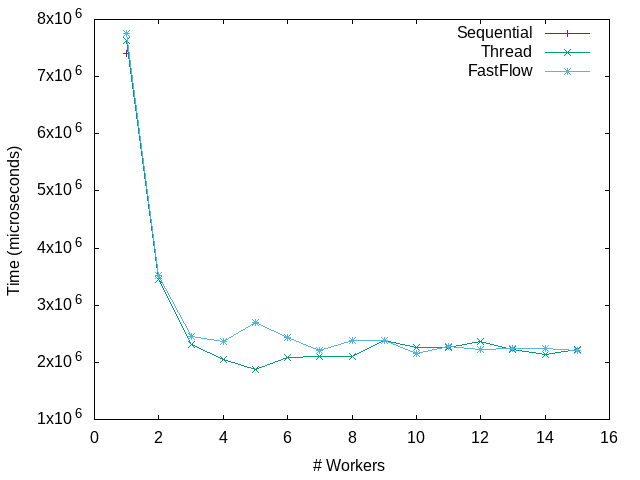
\includegraphics[width=\linewidth]{img/local_20_10000_100_rand_t.png}
        \caption{Local time with 20 nodes, 10000 elements of population and 100 iterations}
        \label{fig:local_time}
    \end{figure}

    \section{Performance: remote analisy}\label{sec:s4}
	Something weird happens when we try to measure the same thing on the remote machine
\end{document}


% \textbf{Micro-Recall}

            %\begin{figure}
                %\includegraphics[width=\linewidth]{../experiments/acp/no_onehot.png}
                %\caption{Training plot for acp task with only two classes [positive, negative]}
                %\label{fig:train-acd-no-onehot}
            %\end{figure}
                %\begin{figure}
                %\includegraphics[width=\linewidth]{../experiments/acp/without_preprocessing.png}
                %\caption{Training plot for acp task with 3 output neurons, but embeddings coverage of 85\% instead of 95\%}
                %\label{fig:train-acd-no-preprocessing}
            %\end{figure}


% $micro-recall$ and $f1-score$.


%        \begin{table}[h!]
%            \begin{center}
%                \caption{element for class}
%                \label{tab:table1}
%                \begin{tabular}{l|c|c|c|r}
%                    \textbf{data} & \textbf{positive} & \textbf{neutral} & \textbf{mixed} & \textbf{negative}\\
%                    \hline
%                        train & 4942 & 0 & 173 & 3797\\
%                        test & 2080 & 0 & 64 & 1757\\
%                \end{tabular}
%            \end{center}
%        \end{table}
